\documentclass{article}

\usepackage{arxiv}

\usepackage[utf8]{inputenc} % allow utf-8 input
\usepackage[T1]{fontenc}    % use 8-bit T1 fonts
\usepackage{hyperref}       % hyperlinks
\usepackage{url}            % simple URL typesetting
\usepackage{booktabs}       % professional-quality tables
\usepackage{amsfonts}       % blackboard math symbols
\usepackage{microtype}      % microtypography
\usepackage{graphicx}
\usepackage{natbib}
\usepackage{doi}
\usepackage{listings}



\title{Scalable machine learning pipelines for waterbody delineation, classification, and change detection}

%\date{September 9, 1985}	% Here you can change the date presented in the paper title
\date{} 					% Or removing it

\author{ \href{https://orcid.org/0000-0002-5924-2464}{
\includegraphics[scale=0.06]{orcid.pdf}\hspace{1mm}Jemma Stachelek}, Charles J. Abolt, Jon Schwenk \\
	Earth and Environmental Sciences\\
	Los Alamos National Laboratory\\
	Los Alamos, NM, USA, 87544 \\
	\texttt{jsta@lanl.gov} \\
}

% Uncomment to remove the date
%\date{}

% Uncomment to override  the `A preprint' in the header
\renewcommand{\headeright}{\href{https://doi.org/}{DOI: 10.000/XXXXX}}
\renewcommand{\undertitle}{This is a draft of a Manuscript in preparation for publication in Geophysical Research Letters \href{https://doi.org/10.1000/XXXXX}{DOI: 10.1000/XXXXX}}
\renewcommand{\shorttitle}{ML pipelines for waterbody imagery}

%%% Add PDF metadata to help others organize their library
%%% Once the PDF is generated, you can check the metadata with
%%% $ pdfinfo template.pdf
\hypersetup{
pdftitle={Scalable machine learning pipelines for waterbody delineation, classification, and change detection},
pdfsubject={stat.AP},
pdfauthor={Jemma Stachelek}
}

\begin{document}
\maketitle

\begin{abstract}
	This is an Abstract.
\end{abstract}

\section{Introduction}
This work was built upon a previous effort \citep{stachelek_hydroml}.

\section{Methods}

\subsection{Data description}

We used some data

\subsection{Model overview}

It was modeled with an equation:

\begin{equation}
	pdf(A) = \alpha x_{min}^{\alpha}A^{-(\alpha+1)} \\
	\label{eqn:pareto_pdf}
\end{equation}

\section{Results}

\begin{figure}
	\centering
	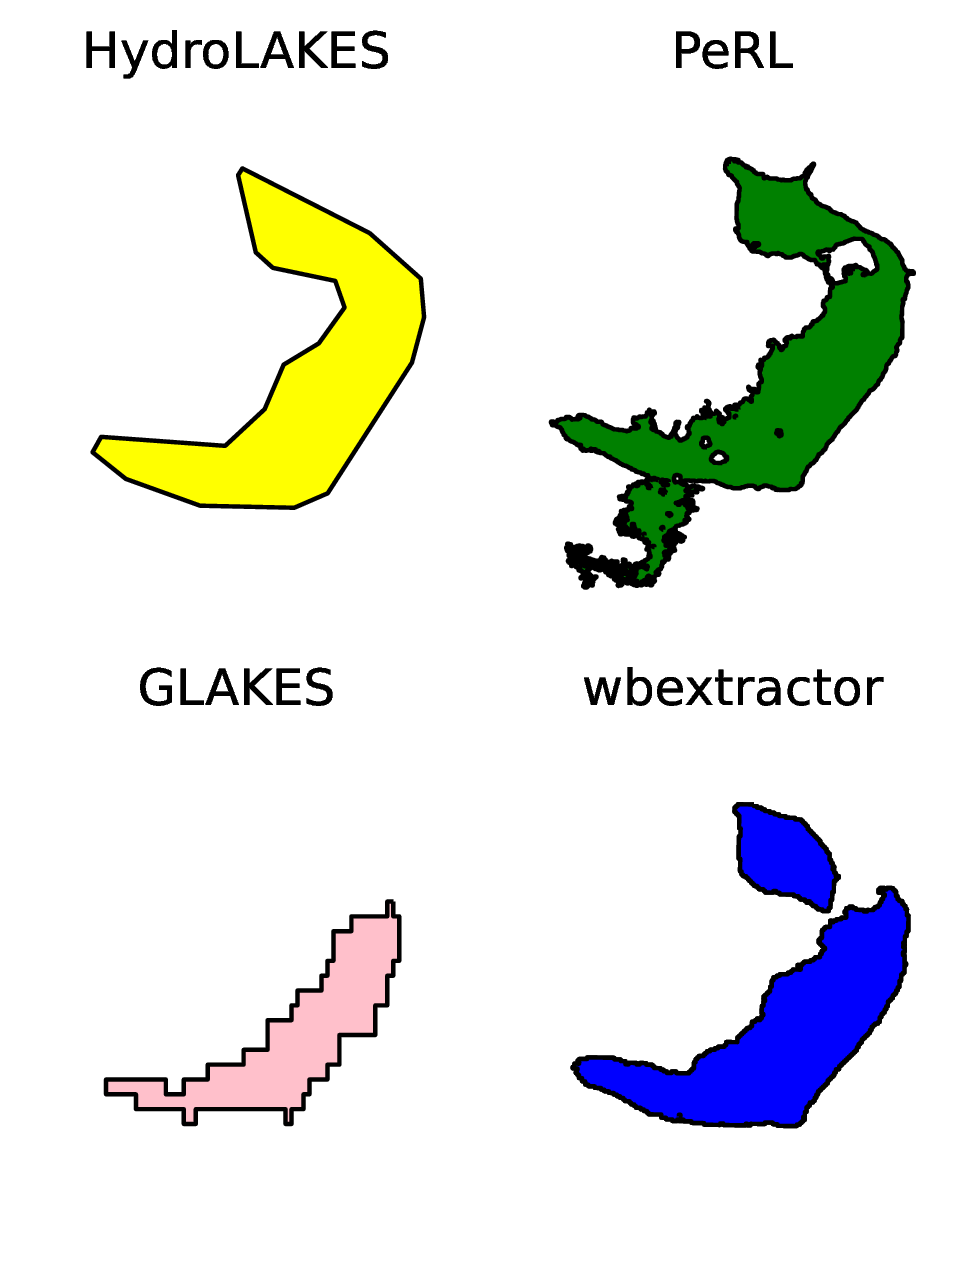
\includegraphics{../figures/single_wb}
	\caption{This is a caption}
	\label{fig:single_wb}
\end{figure}

\section{Discussion}

We have a discussion section.

\section{Data Availability Statement}

All data and code associated with this manuscript are available at: \href{https://doi.org}{https://doi.org}

\section{Acknowledgements}

This work was supported by Los Alamos National Laboratory (LDRD-20220697PRD1).

\bibliographystyle{jsta}
\bibliography{riverlakeid}

\end{document}
